\documentclass[]{article}
\usepackage{proceed2e}

\RequirePackage[OT1]{fontenc}
\RequirePackage{amsthm,amsmath}
\RequirePackage[numbers]{natbib}
\RequirePackage[colorlinks,citecolor=blue,urlcolor=blue]{hyperref}

\usepackage{amsfonts}
\usepackage{algorithm2e}
\usepackage{caption}
\usepackage{subcaption}
\usepackage{graphicx,xcolor}
\usepackage{subcaption}
\usepackage{tikz}
\usetikzlibrary{positioning}

% Standard operators.
\DeclareMathOperator*{\argmin}{arg\,min}
\DeclareMathOperator*{\argmax}{arg\,max}
\DeclareMathOperator{\sign}{sign}

% Standard commands.
\newcommand{\paren}[1]{\left({#1}\right)}
\newcommand{\brac}[1]{\left[{#1}\right]}
\newcommand{\set}[1]{\left\{{#1}\right\}}
\newcommand{\abs}[1]{\left|{#1}\right|}
\newcommand{\norm}[1]{\abs{\abs{{#1}}}}
\newcommand{\E}[1]{\mathbb{E}\brac{{#1}}}
\newcommand{\V}[1]{\mathbb{V}\brac{{#1}}}
\renewcommand{\Pr}[1]{\mathbb{P}\brac{{#1}}}
\newcommand{\R}{\mathbb{R}}


% Custom commands.
\newcommand{\1}{\mathbf{1}}
\newcommand{\0}{\mathbf{0}}
\newcommand{\X}{\mathcal{X}}
\newcommand{\x}{\mathbf{x}}
\newcommand{\y}{\mathbf{y}}
\renewcommand{\O}[1]{\mathcal{O}\paren{{#1}}}
\newcommand{\ang}[1]{\left\langle{#1}\right\rangle}

% Custom environments
\newtheorem{theorem}{Theorem}[section]
\newtheorem{lemma}[theorem]{Lemma}
\newtheorem{proposition}[theorem]{Proposition}
\newtheorem{corollary}[theorem]{Corollary}


\title{Adaptive Neural Network Representations for Parallel and Scalable Bayesian Optimization}

% The author names and affiliations should appear only in the accepted paper.
\author{ {\bf James Brofos} \\
Dartmouth College\\
Hanover, NH 03755 \\
\And
{\bf Rui Shu} \\
Dartmouth College\\
Hanover, NH 03755 \\
\And
{\bf Matthew Jin} \\
Dartmouth College\\
Hanover, NH 03755 \\
}

\begin{document}

\maketitle

\begin{abstract}
	Bayesian optimization has emerged as a powerful, new technique for interpolating and optimizing a wide range of functions which are expensive to compute. The primary tool of Bayesian optimization is the Gaussian process, which permits the investigator to define a prior belief, which is then transformed into a posterior through sequential sampling of points. Unfortunately, Gaussian process interpolation suffers from a major computational bottleneck that makes it prohibitively expensive to utilize in large-scale optimization routines. In this work, we investigate the use of deep neural networks for learning a representation of the space for which a much less computationally expensive interpolation algorithm may be used. Our implementation adaptively updates the representation of the neural network as more data becomes available over time. Since this neural network-based approach is parallelizable, we are able to exploit simultaneous function evaluation and network parameter learning. We show that this neural network-based approach leads to many of the same appealing properties of Gaussian processes, and which scales only linearly in the number of observations \textit{ceteris paribus}.
    
    We additionally seek to provide a theoretical explanation regarding \textit{why} an optimization algorithm of this form functions at all. For this, we develop a probabilistic theory of martingales and apply it to the cumulative regret incurred by the neural network-based approach to Bayesian optimization. We find that the performance of the deep neural network is consistent with the predictions of our probabilistic theory. We therefore speculate on the kind of representation that is learned by the network in its final hidden layer. We also show that our approach is easily extended to a parallel situation, which results in faster optimization. Numerical experiments demonstrate the efficacy of using deep networks for learning representations amenable to computationally inexpensive interpolation methods.
\end{abstract}

\section{Introduction}

Modern machine learning algorithms are dependent on hyperparameter tuning to increase their performance. Recently Bayesian optimization, wherein the hyperparameter space of the model is interpolated by a Gaussian process, has been recognized as a popular methodology for online hyperparameter tuning. To select the next hyperparameter configuration in this  setting, one can maximize an \textit{acquisition function} such as the expected improvement or greatest confidence bound. The acquisition function incorporates knowledge of the posterior mean and variance to derive a quantifiable exploration-exploitation trade-off at every point in the hyperparameter space. Bayesian optimization performs an intermediate maximization over the acquisition function criterion to determine the next experimental configuration of the hyperparameters to evaluate.

In Bayesian optimization the goal is to optimize a black-box function $f:\X\to \R$, where $\X$ is a compact subset of the unit hypercube. Bayesian optimization models $f$ as a (possibly noisy) Gaussian process, wherein uncertainty is captured by a conditional normal distribution at every point $\x\in\X$. Given a set of inputs in $\X$ and responses from $f$, we can condition the Gaussian process on the set of tuples $\set{\paren{\x_i,y_i}}_{i=1}^n$ for $n\in\mathbb{N}$. The mean and variance of the posterior Gaussian process interpolation are provided to the acquisition function to make an informed decision which point of $\X$ to next query.

Bayesian optimization is especially useful when $f$ is expensive to compute, taking perhaps hours or days to complete. Examples of functions fitting into this category include Gaussian mixture models, wherein $\x$ represents the number of clusters to fit and $f\paren{x}$ is the BIC of the Gaussian mixture for some fixed data set. For problems of this form, hyperparameter optimization which assumes the form of a grid-search through $\X$ quickly become intractable. Hence, it is necessary to have a means of inferring the behavior of $f$ and through which intelligent and sequential point selection can be attained. Gaussian processes have traditionally filled this role throughout the Bayesian optimization literature.

Bayesian optimization classically imposes some assumptions on the functional form of $f$. Namely, $f$ is said to be drawn from a Gaussian process $\mathcal{G}\mathcal{P}\paren{m, k}$ with mean function $m : \X\to\R$ and covariance function (also called the \textit{kernel function}) $k : \X\times\X \to\R_+$. It can be shown that without loss of generality, the mean can be taken to be zero for every point of $\X$ as the Gaussian process can be completely parametrized by the covariance function. 

More specifically, Bayesian optimization represents a methodology for solving the maximization task,
\begin{eqnarray}
	\label{eq:opti}
	\x^\star = \argmax_{\x\in\X} f\paren{\x}.
\end{eqnarray}
The efficiency of an optimization algorithm and its ability to balance exploitation with exploration is measured cumulatively for each sequential point selection. We use the \textit{empirical cumulative regret} to evaluate the performance, which is defined at the $n^{\text{th}}$ iteration to be the quantity,
\begin{eqnarray}
	R_n = \sum_{i=1}^n f\paren{\x^\star} - f\paren{\x_i},	
\end{eqnarray}
where $\x_i\in \X$ is the point sampled at the $i^{\text{th}}$ iteration of the algorithm. We additionally report the performance of our neural network-based optimization in terms of the \textit{empirical minimum regret}. The minimum regret is the best performance of the algorithm on all query points at the $n^{\text{th}}$ iteration; more formally,
\begin{eqnarray}
	Q_n = \min_{i\in\brac{n}}\set{f\paren{\x^\star} - f\paren{\x_i}}.
\end{eqnarray}

The aim of this research is to solve the optimization problem in Equation \ref{eq:opti} without relying on a Gaussian process infrastructure. The motivation behind this being that Gaussian processes are not scalable as more information is obtained from $f$ (for a more thorough explanation of this limitation, refer to Section \ref{sec:deep-lear-arch-regr}). Following the work of \cite{snoek-scalable}, we investigate the use of deep learning architectures for learning a representation of the hyperparameter space which is related linearly with the output of $f\paren{\x}$ for any $\x\in\X$. 

In Section \ref{sec:back-prio-work} we discuss the recent literature on Bayesian optimization and recent techniques that have emerged as being useful for query point selection. We then discuss how a neural network may learn representations and how these representations may be used to interpolate the hyperparameter space in Section \ref{sec:deep-lear-arch-regr}. Some theoretical justification regarding why the optimization procedure works is provided in Section \ref{sec:theo-boun}. We finally evaluate the performance of our neural network-based approach in Section \ref{sec:expe-resu} on a collection of real and synthetic machine learning problems. We find our approach to parameter optimization to be highly effective in practice and suggest it as an alternative to Gaussian process optimization when scalability becomes a concern. 



\section{Background and Prior Work}
\label{sec:back-prio-work}

% James - edited. Should re-read.
Our work centers around the use of neural network regression. Neural network regression is an interpolation algorithm such that for some input hyperparameter $\x$ outputs a prediction $\hat{y}$, where $\hat{y}$ is an estimate for some expensive black-box function $f\paren{\x}$. The neural network's prediction is generated by simply feeding $\x$ forward through the network using weights that are learned via backpropogation and stochastic gradient descent. In practice, neural network regression may be used to generate a regression estimate for a learning algorithm's performance on a test data set as a function of a set of hyperparameters.

In the context of this paper, rather than feed each training set element $\x_i$ through the entire network to generate some prediction $y_i$, we instead output the representation $\nu(x_i)$, which consists of the values of the nodes in the final hidden layer of the neural network. The set of all $\nu(x_i)$ is then regressed on using ordinary least squares to generate a predictor which, in conjunction with an acquisition function such as expected improvement, allows us to decide the next point to query.

Our experiments use the \textit{expected improvement} criterion, which has an appealing closed-form and natural intuition. The expected improvement measures how much the function value $f\paren{\x}$ can be expected to improve over the current best function evaluation $f\paren{\x_{\text{best}}}$. For any $\x\in\X$ we define the quantity,
\begin{eqnarray}
	\gamma\paren{\x} = \frac{\mu\paren{\x ; \set{\paren{\x_i,y_i}}_{i=1}^n} - f\paren{\x_{\text{best}}}}{\sigma\paren{\x ; \set{\paren{\x_i,y_i}}_{i=1}^n}},
\end{eqnarray}
where $\mu\paren{\cdot;\cdot}$ and $\sigma\paren{\cdot;\cdot}$ are the posterior mean and variance, respectively. From here, expected improvement is computed to be the quantity,
\begin{eqnarray}
	\sigma\paren{\x ; \set{\paren{\x_i,y_i}}_{i=1}^n}\paren{\gamma\paren{\x}\Phi\paren{\gamma\paren{\x}} + \phi\paren{\gamma\paren{\x}}},
\end{eqnarray}
where $\Phi\paren{\cdot}$ and $\phi\paren{\cdot}$ are the cumulative and probability density functions of a standard normal random variable, respectively. In addition to the expected improvement, other common acquisition criteria include \textit{probability of improvement} ($\Phi\paren{\gamma\paren{\x}}$) and \textit{greatest confidence bound} ($\mu\paren{\x;\set{\paren{\x_i,y_i}}_{i=1}^n} + \kappa_n \sigma\paren{\x;\set{\paren{\x_i,y_i}}_{i=1}^n}$, for $\kappa_n > 0$).

Recent work has empirically shown that the expected improvement has better performance capabilities than does the probability of improvement. Moreover, unlike the greatest confidence bound, there is not an acquisition hyperparameter that must be tuned. The expected improvement represents an appealing non-parametric choice and is therefore the focus of these results.

Recently, much research has been devoted to the study of Gaussian process optimization, including substantial theoretical results, distributed optimization, practical considerations in Bayesian optimization, constrained optimization, and the application of reversible learning to hyperparameter selection. Gaussian processes can be classically considered as defining a distribution over functions; this usage makes them popular in the Bayesian optimization setting due to their desirable analytic, adaptable, and closed-form uncertainty properties. Recent research has focused on scaling Gaussian processes to high-dimensional optimization problems, as well as augmenting the standard approach through the incorporation of Monte Carlo simulations of the response variable and slice sampling.

\begin{figure*}
\centering
\begin{subfigure}[b]{0.3\textwidth}
	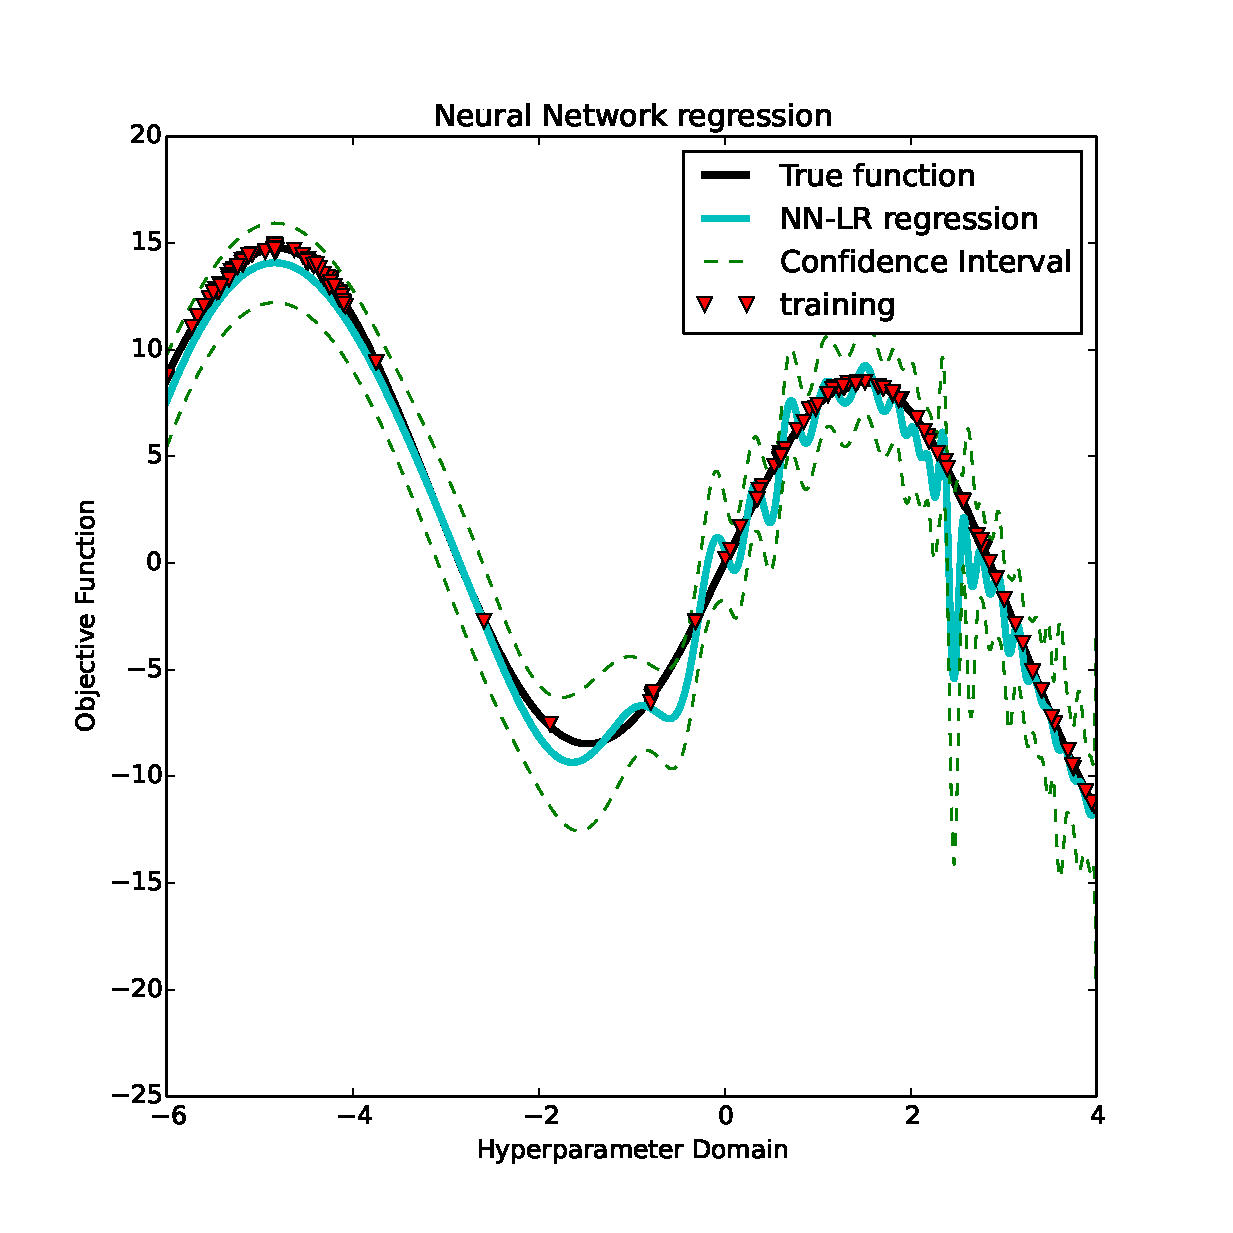
\includegraphics[width=\textwidth]{images/regression.eps}
    \caption{Network Regression}
 	\label{fig:regr}
\end{subfigure}
~ 
\begin{subfigure}[b]{0.3\textwidth}
	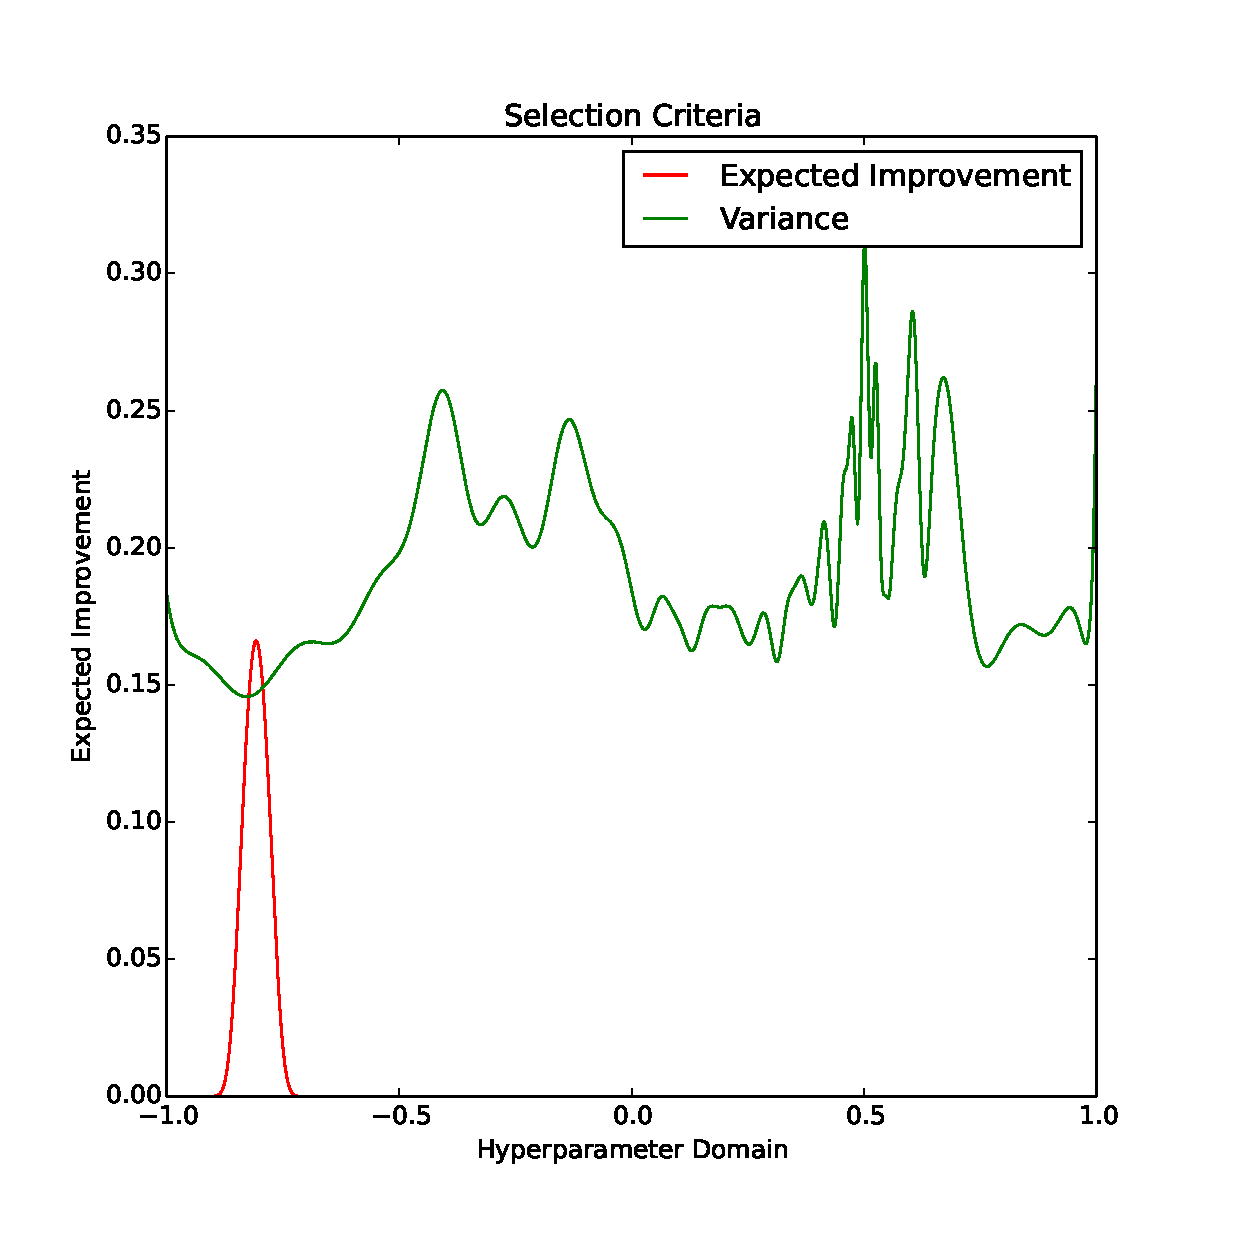
\includegraphics[width=\textwidth]{images/expected_improvement.eps}
	\caption{Acquisition Functions}
	\label{fig:expe_impr}
\end{subfigure}
~
\begin{subfigure}[b]{0.3\textwidth}
	\def\layersep{1cm}
    \hspace*{-0.5em}\raisebox{2em}{
	\begin{tikzpicture}[shorten >=1pt,->,draw=black!50, node distance=\layersep, scale=0.6]
    \tikzstyle{every pin edge}=[<-,shorten <=1pt]
    \tikzstyle{neuron}=[circle,fill=black!25,minimum size=10pt,inner sep=0pt]
    \tikzstyle{input neuron}=[neuron, fill=green!50];
    \tikzstyle{output neuron}=[neuron, fill=red!50];
    \tikzstyle{hidden neuron}=[neuron, fill=blue!50];
    \tikzstyle{annot} = [text width=4em, text centered]

    % Draw the input layer nodes
    \foreach \name / \y in {1,...,4}
    % This is the same as writing \foreach \name / \y in {1/1,2/2,3/3,4/4}
        \node[input neuron,pin=left:$x_\y$] (I-\name) at (0,-\y) {};

    % Draw the hidden layer nodes
    \foreach \name / \y in {1,...,5}
        \path[yshift=0.5cm]
            node[hidden neuron] (H1-\name) at (\layersep,-\y cm) {};
	% Draw the hidden layer nodes
    \foreach \name / \y in {1,...,5}
        \path[yshift=0.5cm,xshift=1.3cm]
            node[hidden neuron] (H2-\name) at (\layersep,-\y cm) {};
	% Draw the hidden layer nodes
    \foreach \name / \y in {1,...,5}
        \path[yshift=0.5cm,xshift=2.6cm]
            node[hidden neuron] (H3-\name) at (\layersep,-\y cm) {};


    % Draw the output layer node
    \node[output neuron,above right=-0.27cm and .4cm of H3-3,pin={[pin edge={->}]right:$\hat{y}$}] (O) {};

    % Connect every node in the input layer with every node in the
    % hidden layer.
    \foreach \source in {1,...,4}
        \foreach \dest in {1,...,5}
            \path (I-\source) edge (H1-\dest);
    \foreach \source in {1,...,5}
        \foreach \dest in {1,...,4}
            \path (H1-\source) edge (H2-\dest);
    \foreach \source in {1,...,5}
        \foreach \dest in {1,...,4}
            \path (H2-\source) edge (H3-\dest);

    % Connect every node in the hidden layer with the output layer
    \foreach \source in {1,...,5}
        \path (H3-\source) edge (O);

    % Annotate the layers
    \node[annot,above of=H2-1, node distance=1cm] (h2) {\tiny{Tanh Hidden Layers}};
    \node[annot,left of=h2] (h1) { };
    \node[annot,right of=h2] (h3) { };
    \node[annot,left of=h1] {\tiny{Input Layer}};
    \node[annot,right of=h3] {\tiny{Linear Output Layer}};
\end{tikzpicture}
	}
	\caption{Network Architecture}
	\label{fig:arch}
\end{subfigure}
\caption{An illustration of our proposed optimization algorithm showing in \ref{fig:regr} the interpolation using the neural network's representation at the last hidden layer and in \ref{fig:expe_impr} the selection criteria (expected improvement and greatest variance) used to identify the next query point. Using linear regression we obtain confidence envelopes about the predicted mean, which are necessary for weighing the exploitation-exploration trade-off. In \ref{fig:arch} we shown a \textit{scaled down} version of the architecture used in our experiments: namely, our approach can handle more than four inputs to $f$ and each hidden layer uses fifty (rather than five) hidden units. However, the architecture shown here is at least illustrative of the overall optimization algorithm. The weights connecting the last hidden layer are replaced by those learned via linear regression \textit{post hoc}.}
\label{fig:regr-expe-impr-arch}
\end{figure*}

\section{Deep Learning Architectures and Regression}
\label{sec:deep-lear-arch-regr}

An important limitation of Gaussian processes regression is that updating the posterior belief is a cubic computation in the number of observations. In particular, the major computational bottleneck in the update equation comes from the inversion of an $n\times n$ kernel matrix. In this work we are interested in practical methods for large-scale Bayesian optimization. 

Linear regression represents the simplest form of interpolation in the modern statistics literature. In this model, a target variable is assumed to be a linear combination of some underlying set of model covariates. Under the assumptions of the model, it is possible to compute standard errors of the coefficients and confidence intervals for a point prediction made by the interpolant. 

Supposing that $\y = \mathbf{X}\beta + \boldsymbol{\epsilon}$ for $\mathbf{X}\in\R^{n\times k}$, then it can be inferred from the linear regression normal equation that the least squares estimator of $\beta$ is obtained by inverting a $k\times k$ matrix. This operation has the desirable property of of scaling linearly in the number of observations $n$ and cubically in the number of covariates. 

We therefore use a neural network to learn a $k$-dimensional representation of $\x$ which is \textit{linearly} related to the response variable. In particular, we use the last hidden layer of the neural network, which, if learning was successful, can undergo a weighted sum of the activations in each hidden unit to estimate the target. The neural network also has an advantage in the sense that it is unnecessary to learn the parameters of the classical Gaussian process kernel via maximum likelihood. Parameter learning in this sense is computationally difficult, since closed-form solutions for the maximum likelihood estimates do not exist and gradient ascent algorithms are oftentimes ill-behaved.

More specifically, we propose to learn a network with $k$ hidden layers and $l$ hidden units per layer. The hyperparameter configuration $\x$ (which we had assumed early had a compact support in the unit hypercube) is provided to the input layer of the neural network. We represent the response as $y=f\paren{\x}$ and this value is interpolated by a single neuron at the output layer of the neural network. Let $g_i\paren{\x}$ be the feed-forward process by which an input $\x$ to the neural network is mapped to the value in the $i^\text{th}$ hidden unit in the last hidden layer. Taken as a column, the $l$-dimensional vector $\set{g_i\paren{\x}}_{i=1}^l$ gives the neural network's learned representation of the input, which is linearly related with the response variable to be maximized. We therefore see that the functions $g_i\paren{\cdot}$ depend crucially on the learned parameters of the neural network. These parameters are trained using backpropogation and stochastic gradient descent. The activation functions of the neural network are hyperbolic tangent functions for the hidden layers, but the output layer makes use of a linear activation. 

For notational simplicity, let $\mathcal{D} = \set{\paren{\x_i,y_i}}_{i=1}^n$ be the set of hyperparameters and associated responses for the first $n$ training examples obtained by sampling $f$. Then it is possible to use the neural network to transform $\x_i$ into a representation that is linearly related to $y_i$. This is achieved by feeding $\x_i$ forward in the deep neural network until it reaches the last hidden layer. We denote by $\boldsymbol{\Phi}$ the $n\times l$ matrix created by feeding $\x_i$ through the network for every $i\in\brac{n}$ and concatenating the representations. Then the predictive mean and variance using the learned representation of the neural network are,
\begin{eqnarray}
	\mu\paren{\x;\mathcal{D}} &=& \paren{\paren{\boldsymbol{\Phi}^T\boldsymbol{\Phi}}^{-1}\boldsymbol{\Phi}^T\y}^T \nu\paren{\x} ~~~\\
    \sigma^2\paren{\x;\mathcal{D}} &=& \hat{\sigma}^2 \paren{1+\mathcal{G}},
\end{eqnarray}
where $\nu\paren{\x}= \paren{g_1\paren{\x}, \ldots, g_l\paren{\x}}^T$ and $\hat{\sigma}^2$ is the maximum likelihood estimate of the amount of noise present in the linear relationship between $\y$ and $\boldsymbol{\Phi}$ and,
\begin{eqnarray}
	\mathcal{G} = \nu\paren{\x}^T\paren{\boldsymbol{\Phi}^T\boldsymbol{\Phi}}^{-1}\nu\paren{\x}.
\end{eqnarray}
 

Replacing the weights connecting the last hidden layer of the network with the linear output layer is advantageous since it allows us to capture uncertainty in the final layer's weights via the usual assumptions of linear regression. Unlike other methods of regression, such as Bayesian linear regression or $\ell_1$-regularization, vanilla linear regression benefits from being without hyperparameters of its own to tune. We also find that when, as in the early states of sampling $f$, there is little training data, it is often the case that the neural network does not learn an effective interpolant of the hyperparameter space. However, empirically, it is the case that the representation contained in the last hidden layer are informative in the sense that their weighted sum can be taken to produce a mean function with low squared error. 




\subsection{Model and Optimization Details}
\label{sec:mode-and-opti-deta}

Obviously when the dimension of the neural network's representation exceeds the number of samples thus far, linear regression leads to a degenerate matrix inversion. As a result of this, we sample a number of points equal to the number of hidden units in the final hidden layer of the network. 

The expected improvement criterion may conceivably be negative throughout the support of the hyperparameter space when the optimization procedure becomes quite sure of its identified maximum. In other words, every point in $\X$ is expected to lead to a function evaluation $f\paren{\x}$ which will not exceed the current maximum. When this occurs, we change our point selection strategy to pursue pure exploration. This amounts to querying that point for which the prior variance estimate is largest. 

\subsection{Parallel Optimization Structure}

We augment the neural network optimization model by incorporating parallel function evaluations and network learning. In many settings, it may be desirable to use a system wherein batches of parameter configurations, $\set{\x_i}_{i=1}^m$ are evaluated in parallel. In the design of our parallel representation learning, we consider a \textit{high-throughput} wherein each of the $m$ configurations to evaluate are delegated to separate processes and the response feedback is obtained asynchronously as each experiment is completed.

In practice, we adopt the master-worker parallelization paradigm. This means that one process -- the eponymous master process -- is devoted to selection of individual query points, which are then assigned to individual worker processes. The worker processes, upon receiving the selected hyperparameter configurations from the master process, then perform the expensive function evaluation of $f$. We augment this process by relearning the representation of the hyperparameter space as more information about the relationship between the domain and range of $f$ become available. In particular, after $n$ observations  have been observed since the last time the network was learned, a single worker process is tasked with performing backpropogation and stochastic gradient descent to train the parameters of the neural network. These parameters are then broadcast to the master process, which makes use of them in all subsequent representation and regression tasks.


\section{Theoretical Bounds}
\label{sec:theo-boun}

%To do: Email Balkcom, put our work on the d-mouth technical reports website. Include sentence acknowledging that work (here) and also add a citation/link to the work in the biblio
We seek now to provide some theoretical justification for why an algorithm of this kind should perform well on black-box optimization. We return now to the idea of regret and introduce a formal notion of regret to analyze it more carefully as a random variable using probability theory. In particular, we regret as the difference,
\begin{eqnarray}
  r_i = f\paren{\x^\star} - f\paren{\x_i} | \mathcal{D}_i.  
\end{eqnarray}
Note that we condition on the set of existing data $\mathcal{D}_i$ by the $i^{th}$ iteration. For $n$ total iterations, the cumulative regret and augmented cumulative regret are given respectively by,
\begin{eqnarray}
  R_n &=& \sum_{i=1}^n r_i \\
  M_n &=& \sum_{i=1}^n r_i - \mu\paren{\boldsymbol{\nu}_i} + \mu\paren{\boldsymbol{\nu}^\star} | \mathcal{D}_i.
\end{eqnarray}
We use the notation $\boldsymbol{\nu}$ as shorthand for $\nu\boldsymbol{\x}$ which the representation learned by the neural network on input $\x\in\X$. Superscripts and subscripts on $\boldsymbol{\nu}$ ($\boldsymbol{\nu}^\star$ or $\boldsymbol{\nu}_i$) refer to the representation of the optimal $\x^\star$ or the representation of $i^\text{th}$ hyperparameter query, respectively. We prove a probabilistic bound on the average cumulative regret of the neural network optimization with respect to the number of iterations that have occurred:
\begin{eqnarray}
  \label{eq:resu}
  \Pr{\frac{R_n}{n} > \epsilon} = e^{-\Omega(n)}.
\end{eqnarray}
The proof relies on demonstrating that $(M_n)_{n \in \mathbb{N}}$ is a particular type of martingale with properties that are crucial to the derivation of Equation \ref{eq:resu}. We begin by presenting two relevant lemmas: First, that $(M_n)_{n \in \mathbb{N}}$ is a martingale; and, second, that $(M_n)_{n \in \mathbb{N}}$ is both heavy on left and sub-Gaussian. 


\begin{figure*}
\centering
\begin{subfigure}[b]{0.3\textwidth}
	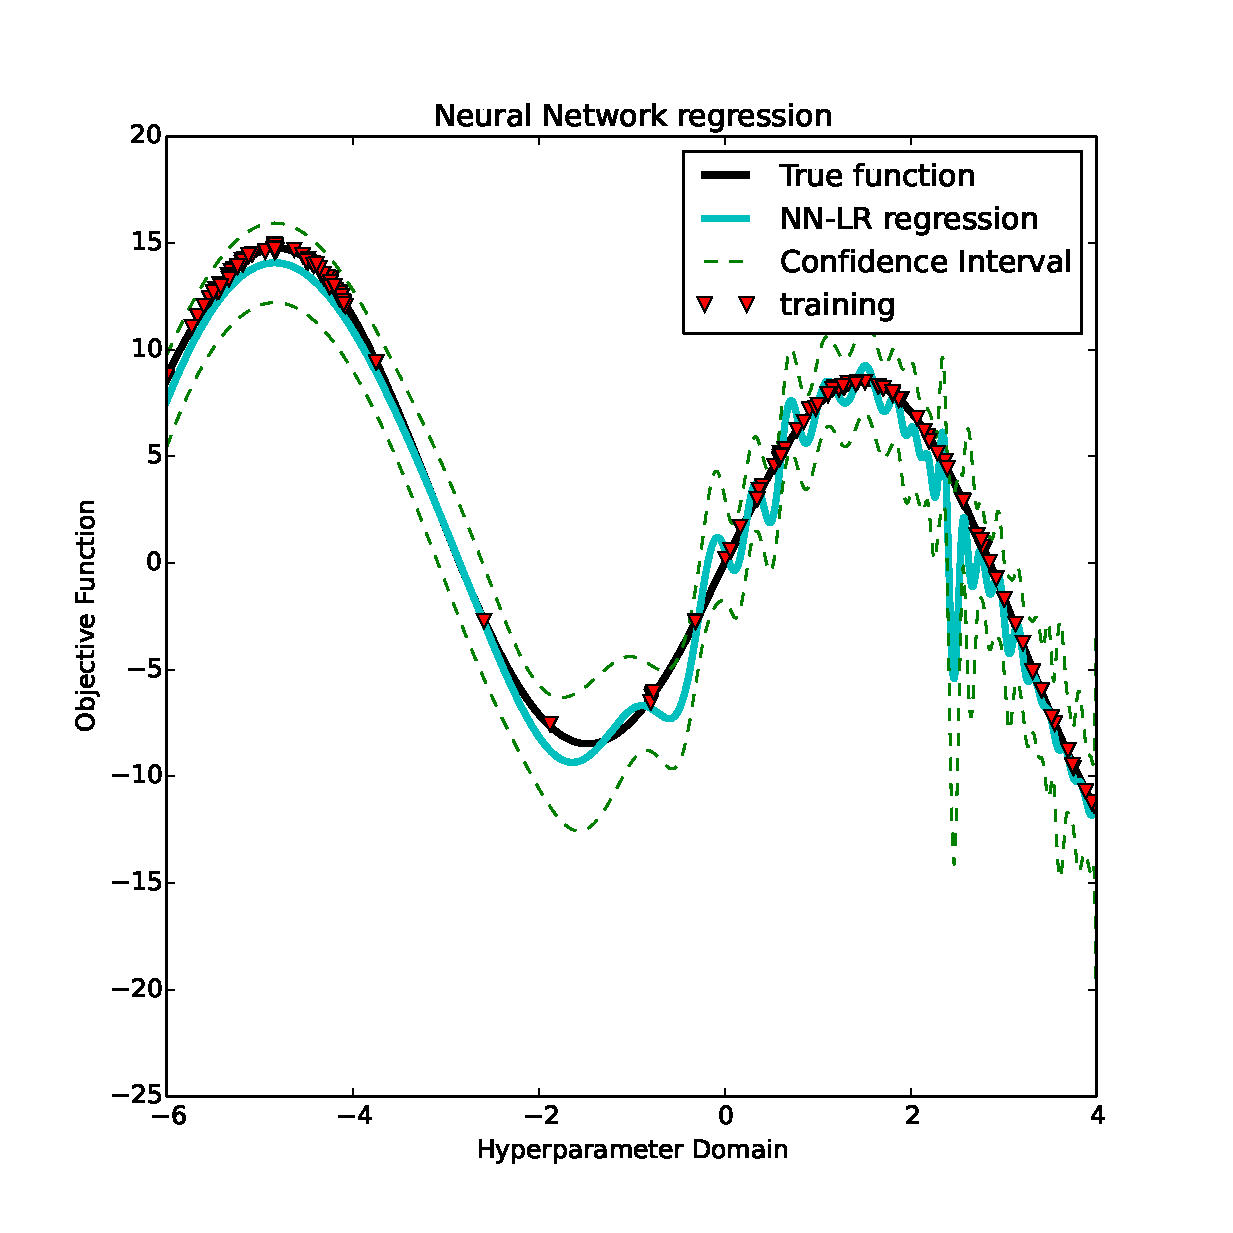
\includegraphics[width=\textwidth]{images/regression.eps}
    \caption{Parallel Speed Increase}
 	\label{fig:para}
\end{subfigure}
~ 
\begin{subfigure}[b]{0.3\textwidth}
	\includegraphics[width=\textwidth]{images/gm.eps}
	\caption{Gaussian Mixture Regret}
	\label{fig:cumu_regr_1}
\end{subfigure}
~
\begin{subfigure}[b]{0.3\textwidth}
	\includegraphics[width=\textwidth]{images/hm.eps}
	\caption{$4$-D Hartmann Regret}
	\label{fig:cumu_regr_2}
\end{subfigure}
\caption{We show an illustration of the speed-up that is possible by exploiting a parallel optimization structure in \ref{fig:para}. In this example, we use four total processes running at parallel: two devoted to evaluating $f$ at the chosen points in $\X$, one for managing work as new information becomes available, and one for updating the neural network representation learned by the neural network as more training data is acquired. In \ref{fig:cumu_regr_1} we show the results of running our neural network-based optimization algorithm on a Gaussian mixture model with multiple modes in the unit hypercube. Additionally in \ref{fig:cumu_regr_2} we show the results of trying to optimize the four-dimensional Hartmann function. Notice that in both cases the optimization successfully finds the global maximum with the function domain as indicated by the minimum regret. Furthermore, the average cumulative regret is trending downwards, as desired.}
\label{fig:para-cumu-regr}
\end{figure*}

\begin{figure}
	\centering
    \captionsetup{width=0.45\textwidth}
    \begin{subfigure}[b]{0.45\textwidth}
		\includegraphics[width=\textwidth]{images/probability_2.eps}
    	\caption{Empirical Probability on Gaussian Process}
    	\label{fig:prob-gaus}
    \end{subfigure}
    
    \begin{subfigure}[b]{0.45\textwidth}
		\includegraphics[width=\textwidth]{images/probability_3.eps}
	    \caption{Empirical Probability on $4$-D Hartmann Function}
		\label{fig:prob-hart}
	\end{subfigure}
	\caption{We show an empirical experiment that demonstrates behavior consistent with the prediction of the theory. In \ref{fig:prob-gaus}, we seek to find the global maximum of a synthetic Gaussian process defined on an interval of $\R$, which is scaled to $\brac{-1,+1}$. The theory implies that for any $\epsilon$ (here $\epsilon = 0.7$), the probability that average regret will exceed $\epsilon$ decreases exponentially for every $n>n_0$, for some $n_0$ dependent on $\epsilon$. We speculate here that $n_0\approx 400$. We run the optimization procedure one-hundred times and calculate empirically the number of times that the average cumulative regret exceeded $\epsilon$ for every $n$. We show the probability on a logarithmic scale and confirm that it does display the exponential decrease. An identical experiment was performed for the (much harder) Hartmann optimization problem in four dimensions. The results are shown in \ref{fig:prob-hart}.}
	\label{fig:prob}
\end{figure}


\begin{lemma}
	The sequence $(M_n)_{n \in \mathbb{N}}$ is a martingale with respect to its difference sequence:
  	\begin{eqnarray}
    	Y_n &=& M_n - M_{n-1} \\
        &=& r_n - (\mu_n\paren{\boldsymbol{\nu}_n} - \mu_n\paren{\boldsymbol{\nu}^\star}) | \mathcal{D}_n.
  	\end{eqnarray}
\end{lemma}
\begin{proof}
	For notational simplity, let $\mathcal{Y}_{n} = \set{Y_i}_{i=1}^{n}$. Realizations of $(M_n)_{n \in \mathbb{N}}$ are contingent on the Bayesian optimization procedure used to find the minimum of $f$. The key insight to understanding the GP update process is recognizing that $f$, conditioned on the presence of data by the $i^{th}$ iteration $\mathcal{D}_i$, is a new Gaussian process: $f|\mathcal{D}_{i} \sim \mathcal{GP}(\mu_i, k_i)$. It is easy, then, letting $\mathcal{Q} = \mathcal{Y}_{n-1}, \mathcal{D}_n$, to see that $\E{Y_n | \mathcal{Y}_{n-1}}$ can simply be written as,
  	\begin{eqnarray}
    	\E{Y_n | \mathcal{Y}_{n-1}} &=& \E{r_n - (\mu_n\paren{\boldsymbol{\nu}_n} - \mu_n\paren{\boldsymbol{\nu}^\star}) | \mathcal{Q}} ~~~~~\\
   		&=& 0.   
  	\end{eqnarray}
  	Crucially, we note that the conditioning on the existing data, $\mathcal{D}_n$, causes the expectation of $f$ to be $\mu_n$. The variance can also be demonstrated to be,
  	\begin{eqnarray}
    	\begin{aligned}
  	 	\V{Y_n | \mathcal{Y}_{n-1}} =& ~~k_n(\x_i, \x_i) + k_n(\x^\star, \x^\star) \\ &- 2k_n(\x^\star, \x_i),
        \end{aligned}
  	\end{eqnarray}
  	simply by computing the variance of $f(\x_i) - f(\x^\star) | \mathcal{D}_n$, which is the difference of two normally distributed random variables. Together, this shows that $Y_N | \set{Y_n}_{n=1}^{N-1}$ is zero-mean and normally distributed. Because this random variable has zero-mean, it can now be shown that $(M_N)_{N \in \mathbb{N}}$ is, in fact a martingale. Indeed, 
  	\begin{eqnarray}
    	\E{M_{n+1} | \mathcal{Y}_n} &=& \E{M_{n} + Y_{n+1} | \mathcal{Y}_n} \\
    	&=& M_n.
  	\end{eqnarray}
  	This completes the proof.
\end{proof}

\begin{lemma}
  	The martingale sequence $(M_n)_{n \in \mathbb{N}}$ is heavy on left, and sub-Gaussian.
\end{lemma}
\begin{proof}
  	We say that a martingale is heavy on left if all its increments are conditionally heavy on left. The increments are heavy on left if it can be shown that
  	\begin{eqnarray}
    	\E{Y_n | \mathcal{Y}_{n-1}} &=& 0.
  	\end{eqnarray}
  	Furthermore,
  	\begin{eqnarray}
    	\E{\min(|Y_n | \mathcal{Y}_{n-1}, a)\sign(Y_n | \mathcal{Y}_{n-1})} &\leq& 0 \label{eq:heav-left}, 
  	\end{eqnarray}
  	for every $a > 0$. Because $Y_n | \mathcal{Y}_{n-1}$ is a zero-mean Gaussian random variable, the above conditions are trivially true. The second condition Equation \ref{eq:heav-left}, in particular, can be shown by exploiting the symmetry of a zero-mean Gaussian distribution. Additionally, we say that the martingale is sub-Gaussian if there exists some $\alpha > 0$ such that for all $n \geq 1$ and $t \in {R}$,
  	\begin{eqnarray}
    	\E{e^{t\cdot Y_n} | \mathcal{Y}_{n-1}} &\leq& e^{\frac{\alpha^2 t^2}{2} \V{Y_n| \mathcal{Y}_{n-1}}}. \label{eq:subg}
  	\end{eqnarray}
  	Since $Y_n | \mathcal{Y}_{n-1}$ is zero-mean Gaussian, it has a well-defined moment-generating function that can be used to show that Equation \ref{eq:subg} is true when we take $\alpha =1$, thus demonstrating that the martingale $(M_n)_{n \in \mathbb{N}}$ is sub-Gaussian.
\end{proof}

\begin{theorem} 
  	We now prove the main result, demonstrating the rapid convergence of the average cumulative regret to zero. In particular,
  	\begin{eqnarray}
    	\Pr{\frac{R_n}{n} > \epsilon} = e^{-\Omega(n)}
  	\end{eqnarray}
\end{theorem}
\begin{proof}
  	There are many existing inequalities known for martingales which are self-normalized with respect to their quadratic variation. For sub-Gaussian, heavy on left martingale such as $(M_n)$, it is known that, for all values $x > 0, a \geq 0, b > 0$,
  	\begin{eqnarray}
    	\begin{aligned}
      	\Pr{\frac{M_n}{a+b\ang{M}_n} \geq x} \\
      	\leq \inf_{p > 1} \set{\E{e^{-(p-1)\frac{x^2}{\alpha^2}\paren{ab + \frac{b^2}{2}\ang{M}_n}}}}^{\frac{1}{p}},
    	\end{aligned}
  	\end{eqnarray}
  	where $\alpha$ (in the case of $(M_n)_{n \in \mathbb{N}}$, $\alpha = 1$) is the value used to satisfy the condition in Equation \ref{eq:subg} and $\ang{M}_n$ is the predictable quadratic variation, given by,
  	\begin{eqnarray}
    	\ang{M}_n &=& \sum_{i=1}^n \E{\paren{M_i - M_{i-1}}^2 | \mathcal{Y}_{n-1}} \\
        &=& \sum_{i=1}^n \V{Y_i | \mathcal{Y}_{n-1}}. 
  	\end{eqnarray}
  	For notational convenience, we shall express $\sum_{i=1}^n \V{Y_i | \mathcal{Y}_{n-1}}$ as $\sum_{i=1}^n \mathbb{V}_i$. To attain a form more amenable to our main result, we set the parameters to be $a = 0, b=n, \alpha=1$. Thus,
  	\begin{eqnarray}
    	\begin{aligned}
    		\Pr{\frac{M_n}{n\ang{M}_n} \geq x} \\
        	\leq \inf_{p > 1} \set{\E{e^{-(p-1)x^2\frac{n^2}{2}\ang{M}_n}}}^{\frac{1}{p}}.
        \end{aligned} \label{eq:conc}
  	\end{eqnarray}
  	The internal expectation expression can quickly be reduced as follows,
  	\begin{eqnarray}
    	\E{e^{-(p-1)x^2\paren{\frac{n^2}{2}\ang{M}_n}}} = \paren{e^{\frac{x^2n^2}{2}\sum_{i=1}^n \mathbb{V}_i}}^{1-p}.
  	\end{eqnarray}
	Thus far, we have dealt purely with the augmented cumulative regret, $(M_N)$, exploiting the known properties of a self-normalized, heavy on left, sub-Gaussian martingale to arrive at the inequality demonstrated in Equation \ref{eq:conc}. To derive an inequality with respect to the cumulative regret, we reduce the augmented cumulative regret into its components, $M_N = R_n - S_n$, where $S_n = \sum_{i=1}^n \mu_i(\x_i) - \mu_i(\x^\star)$. It can now be stated that,
  	\begin{eqnarray}
    	\Pr{\frac{R_n}{n} \geq x\sum_{i=1}^n \mathbb{V}_i + \frac{S_n}{n}} \leq \paren{e^{\frac{x^2n^2}{2}\sum_{i=1}^n \mathbb{V}_i}}^{-\frac{1}{2}}.
  	\end{eqnarray}
	Setting $\epsilon = x \sum_{i=1}^n \mathbb{V}_i + \frac{S_n}{n}$, the derivation of the main result is completed,
  	\begin{eqnarray}
      	\Pr{\frac{R_n}{n} \geq \epsilon} &\leq&
      	\paren{e^{\frac{(n\epsilon-S_n)^2n^2}{2n^2 (\sum_{i=1}^n \mathbb{V}_i)^2 }\sum_{i=1}^n \mathbb{V}_i}}^{-\frac{1}{2}} \\
      	&\leq&
      	\paren{e^{\frac{S_n^2 - 2S_n n \epsilon + n^2\epsilon^2}{2 \sum_{i=1}^n \mathbb{V}_i }}}^{-\frac{1}{2}} \\
      	&=& e^{-\Omega(n)}.
  	\end{eqnarray}
  	This shows the desired result.
\end{proof}

We demonstrated empirically that the neural network-based optimization algorithm is consistent with the predictions of this theory. In particular we calculate the empirical probability that the cumulative regret exceeds $\epsilon$ on two global optimization problems. We observe that in both experiments the probability did decrease exponentially after a particular number of queries had been performed. This result is shown in Figure \ref{fig:prob}. For the Gaussian process in Figure \ref{fig:prob-gaus} the rate of exponential decay is approximately $\frac{-84}{1000}$ while for the Hartmann function in Figure \ref{fig:prob-hart} the rate is approximately $\frac{-12}{1000}$. 

We would therefore like to speculate that the neural network is learning a representation of the hyperparameter space $\X$ such that generally the Gauss-Markov assumptions of ordinary linear regression hold. If then this is true, the martingale properties hold.


\section{Experimental Results}
\label{sec:expe-resu}

Python code for implementing neural network-based learning of hyperparameter representations is made available online at \url{https://github.com/RuiShu/Neural-Net-Bayesian-Optimization}. 

In order to empirically demonstrate the efficacy of the proposed approach, we evaluate its performance on a number of benchmark global optimization problems. In particular, we analyze the performance of the neural network's representation by initializing the optimization procedure with a sample of fifty points drawn uniformly at random from the support of the hyperparameter space.

The first of our experiments involves finding the maximum of a two-dimensional Gaussian mixture. We choose the Gaussian mixture so that it has a multimodal property, which permits us to assess the capability of the algorithm to balance exploitation with exploration. We also implement the four dimensional Hartmann function to evaluate the optimization performance of our approach. The Hartmann function is also multimodal, and it permits us to examine performance on optimization problems with a number of hyperparameters consistent with many modern statistical learning algorithms such as $\ell_1$-regularized regression or SVMs. It has been used as a benchmark by, for instance, Snoek \textit{et al.} \cite{snoek-scalable}.

We compare the empirical average regret, which is the ratio $R_m / m$ for each $m\in\set{ 1,2,\ldots, n}$. Ideally, an optimization algorithm will possess the property that it is asymptotically \textit{no-regret} \cite{srinivas-bandit}: that is, in the limit $\lim_{m\to\infty} R_m / m = 0$. The average regret can be interpreted as a convergence rate for the optimization algorithm, wherein $\argmax_{x\in \set{\x_1,\ldots,\x_n}} f\paren{\x}$ does not deviate from $f\paren{\x^\star}$ by more than the average.

Figure \ref{fig:para-cumu-regr} shows the average and minimum regret obtained by our algorithm on the benchmark problems. We see that generally, by using the expected improvement criterion, the algorithm explores the domain of the function first before honing in on a particular global minimum. This is seen by the initial non-decreasing nature of the average cumulative regret and the eventual attainment of zero minimum regret.

We performed our experiments on a dual-core 2.9 GHz MacBook Pro using in each experiment a total of four processes. Using this computer, optimizing the Gaussian mixture took an average of $104.003$ seconds to perform one-hundred queries; for the Hartmann function, the algorithm took $288.394$ seconds for the same number of queries. 

\section{Conclusion}

In this work, we proposed a distributed methodology for optimizing expensive black box functions through deep learning. In particular, we learn a representation of the hyperparameter space which has a linear relationship with the target variable to be maximized. Unlike earlier approaches using deep learning, our approach does not have additional hyperparameters that must be tuned beyond the network architecture. Because of the nature of linear regression, the computational complexity of interpolation scales linearly in the number of points queries; this is an immense order improvement over the cubic performance of traditional Gaussian process optimization. Our approach also benefits from being fully parallelizable on a computing cluster which leads increased wall-clock time improvements in speed. We demonstrate empirically that our distributed approach achieves competitive performance with state-of-the-art Bayesian optimization procedures.

We were able to demonstrate a theory whose prediction the neural network optimization algorithm appears to obey. 

Several approaches have been considered in the Gaussian process optimization literature for reducing the computational complexity of the full Bayesian update. One method in particular is the Lazy Variance Calculation \cite{desautels}, which avoids the inversion of the $n\times n$ covariance matrix altogether. One direction of future research is to consider similar techniques as this for linear regression, so that the posterior variance can be made, in a sense, to be independent of the response of querying $f$. This could lead to an additional degree of parallelism and a superior distributed exploration-exploitation trade-off. 


\subsubsection*{Acknowledgments}

Our neural networks make use of the Theanets network model regression software, which is itself reliant on the Theano software library. Basic linear algebra, including the computation of the least-squares coefficient estimates, is done using Python's scientific computing package NumPy. Parallelization was implemented using MPI4Py, a Python wrapper for an underlying C implementation of the Message Passing Interface. 

We wish to thank Professor Amit Chakrabarti of Dartmouth College for supervising the independent study by which the authors derived the theoretical results contained herein.


\subsubsection*{References}

\begingroup
\renewcommand{\section}[2]{}
\begin{thebibliography}{}

\bibitem{auer}
Auer, P. Using confidence bounds for exploitation exploration trade-offs. \textit{JMLR}, 3:397–422, 2002.

\bibitem{bercu}
Bercu, B. and Touati, A. Exponential inequalities for selfnormalized martingales with applications. \textit{The Annals of Applied Probability}, 18(5):1848–1869, 2008.

\bibitem{bergstra}
Bergstra, James S., Bardenet, Remi, Bengio, Yoshua, and Kegl, Balazs. Algorithms for hyper-parameter optimization. In \textit{Advances in Neural Information Processing Systems}. 2011.

\bibitem{contal}
Contal, E., Buffoni, D., Robicquet, A., and Vayatis, N. Parallel Gaussian process optimization with upper confidence bound and pure exploration. In \textit{Machine Learning and Knowledge Discovery in Databases}, volume 8188, pp. 225–240. Springer Berlin Heidelberg, 2013.

\bibitem{cover}
Cover, T. M. and Thomas, J. A. \textit{Elements of Information Theory}. Wiley Interscience, 1991.

\bibitem{defreitas}
de Freitas, N., Smola, A. J., and Zoghi, M. Exponential regret bounds for Gaussian process bandits with deterministic observations. In \textit{Proceedings of the 29th International Conference on Machine Learning}. icml.cc / Omnipress, 2012.

\bibitem{desautels}
Thomas Desautels, Andreas Krause, and Joel Burdick. Parallelizing exploration-exploitation tradeoffs with gaussian process bandit optimization. In \textit{International Conference on Machine Learning (ICML)}, 2012.

\bibitem{hensman}
Hensman, J, Fusi, N, and Lawrence, N.D. Gaussian processes for big data. In \textit{Uncertainty in Artificial Intelligence}, 2013.

\bibitem{lee}
Lee, Chen-Yu, Xie, Saining, Gallagher, Patrick, Zhang, Zhengyou, and Tu, Zhuowen. Deeply supervised nets. In \textit{Deep Learning and Representation Learning Workshop}, \textit{NIPS}, 2014.

\bibitem{osborne}
Osborne, Michael A., Garnett, Roman, and Roberts, Stephen J. Gaussian processes for global optimization. In \textit{Learning and Intelligent Optimization}, 2009.

\bibitem{snoek-scalable}
Jasper Snoek, Oren Rippel, Kevin Swersky, Ryan Kiros, Nadathur Satish, Narayanan Sundaram, Md. Mostofa Ali Patwary, Prabhat, and Ryan P. Adams. Scalable Bayesian Optimization Using Deep Neural Networks. \textit{arXiv:1502.05700 [stat.ML]}, 2013. URL \url{http://arxiv.org/abs/1502.05700}.

\bibitem{snoek-practical}
Jasper Snoek, Hugo Larochelle, and Ryan P. Adams. Practical Bayesian optimization of machine learning algorithms. In \textit{Advances in Neural Information Processing Systems (NIPS)}, 2012.

\bibitem{srinivas-bandit}
Niranjan Srinivas, Andreas Krause, Sham Kakade, and Matthias Seeger. Gaussian process optimization in the bandit setting: No regret and experimental design. In \textit{Proceedings of the 27th International Conference on Machine Learning (ICML)}, 2010.

\bibitem{srinivas-bounds}
Srinivas, N., Krause, A., Kakade, S., and Seeger, M. Information-theoretic regret bounds for Gaussian process optimization in the bandit setting. \textit{IEEE Transactions on Information Theory}, 58(5):3250–3265, 2012.

\bibitem{wang}
Wang, Ziyu, Zoghi, Masrour, Hutter, Frank, Matheson, David, and de Freitas, Nando. Bayesian optimization in high dimensions via random embeddings. In \textit{IJCAI}, 2013.

\end{thebibliography}
\endgroup

\end{document}
